\documentclass[a3paper,landscape]{article}

\usepackage[margin=5mm]{geometry}
\pagestyle{empty}
\usepackage{tikz}
\usetikzlibrary{
    decorations.markings,
    decorations.pathmorphing,
    decorations.text,
}
\usepackage{graphicx}
\usepackage{contour}
\contourlength{0.05mm} % important and fragile magic number!

% FONTS
\usepackage{addfont}
\addfont[1]{OT1}{hge}{\textgothic}
\usepackage{fontspec}
\newfontface\textblack{QTHelvet-Black}
\usepackage{cabin}


\begin{document}
    
\noindent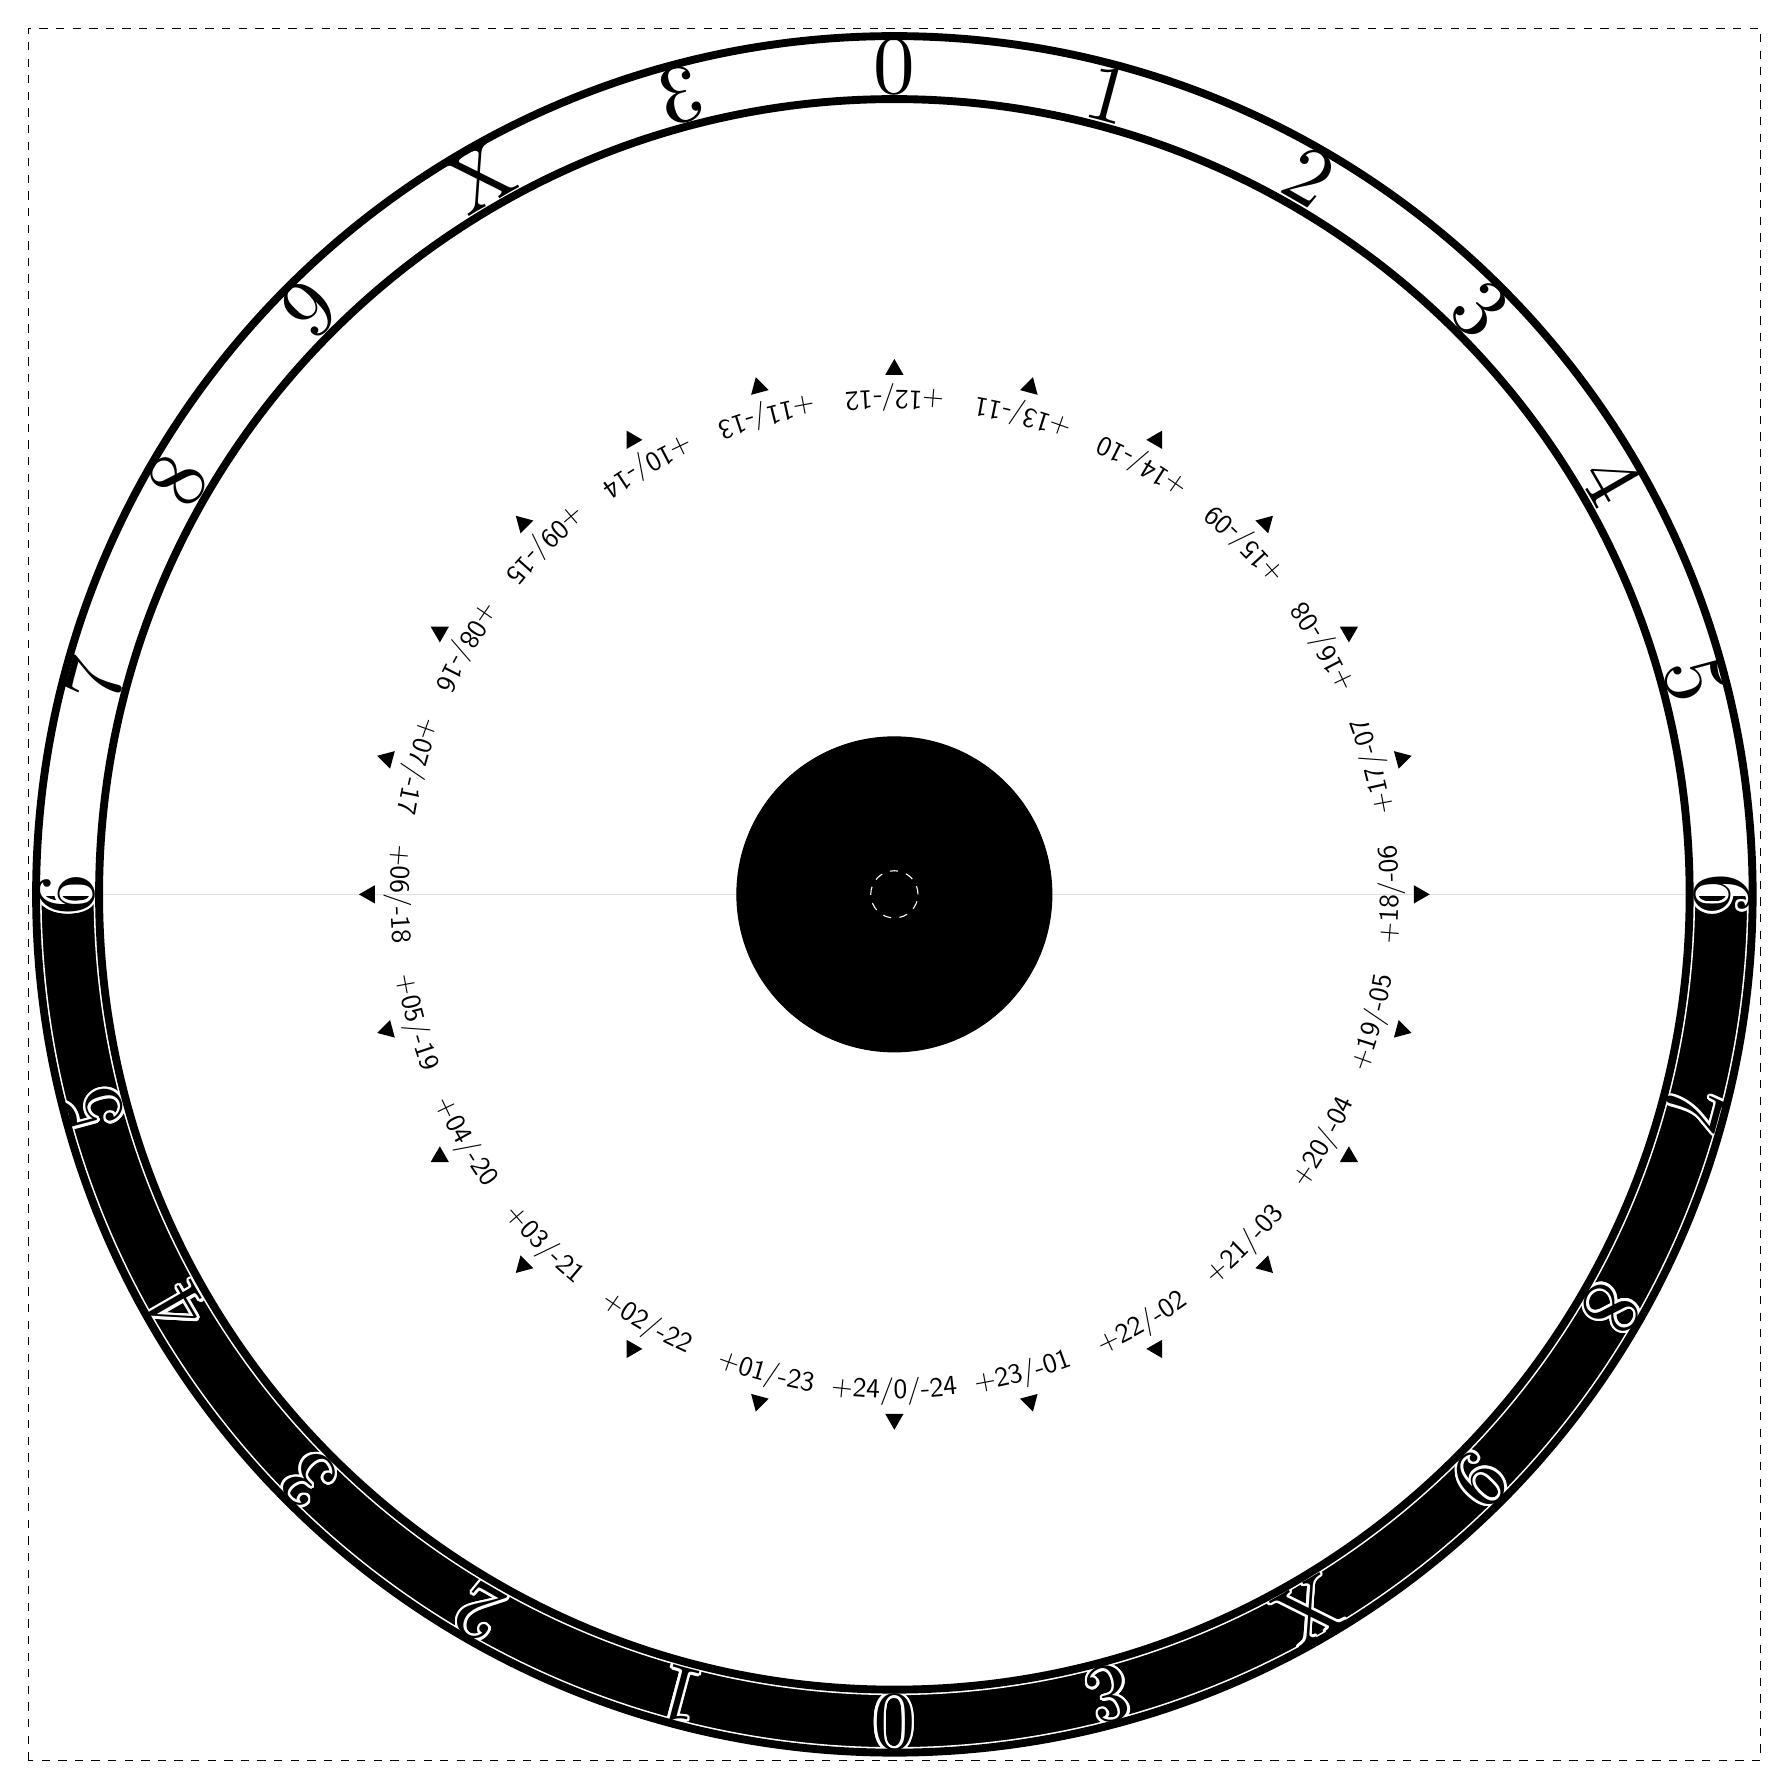
\begin{tikzpicture}
    % BORDER
    \draw[dashed] (-110mm,-110mm) rectangle (110mm,110mm);
    \draw[fill] (0,0) circle [radius=20mm];
    \draw[dashed,white] (0,0) circle [radius=3mm];

    % INNER TIMEZONE ALIGNMENT
    % Timezones
    \foreach [count=\i] \plus/\minus in {%
            01/23,02/22,03/21,04/20,05/19,06/18,%
            07/17,08/16,09/15,10/14,11/13,12/12,%
            13/11,14/10,15/09,16/08,17/07,18/06,%
            19/05,20/04,21/03,22/02,23/01%
    } {
        \path[postaction={decorate,decoration={text align={center},text
            along path,text={|\sffamily|+\plus/-\minus}}}]
            (262.5-15*\i:64mm) arc (262.5-15*\i:277.5-15*\i:64mm);
        \fill (270+15*\i:68mm) -- (271+15*\i:66mm) -- (269+15*\i:66mm);
    }
    \path[postaction={decorate,decoration={text align={center},text
        along path,text={|\sffamily|+24/0/-24}}}]
        (262.5:64mm) arc (262.5:277.5:64mm);
    \fill (270:68mm) -- (271:66mm) -- (269:66mm);
    
    % OUTER RIM
    % Background
    \draw[fill=black,draw=white,line width=.4mm]
        (180:101.5mm) -- (180:108.5mm) arc (180:360:108.5mm)
        (360:108.5mm) -- (360:101.5mm) arc (360:180:101.5mm);
    % Numerals
    \foreach \angle/\label/\xscale in {%
            270/0/1,255/1/1,240/2/1,225/3/1,210/4/1,195/5/1,%
            180/6/1,165/7/1,150/8/1,135/9/1,120/X/1,105/3/-1%
    } {
        \node[rotate=\angle-90,scale=3,inner sep=0pt,xscale=\xscale]
            at (\angle:105mm) {\contour{white}{\label}};
        \node[rotate=\angle+90,scale=3,inner sep=0pt,xscale=\xscale]
            at (\angle-180:105mm) {\contour{white}{\label}};
    }
    % Borders
    \draw [line width=1mm] (0,0) circle [radius=110mm-1mm];
    \draw [line width=1mm] (0,0) circle [radius=100mm+1mm];
\end{tikzpicture}
        
\end{document}
